\documentclass{standalone}
\usepackage{tikz}
\usepackage{ctex,siunitx}
\setCJKmainfont{Noto Serif CJK SC}
\usepackage{tkz-euclide}
\usepackage{amsmath}
\usetikzlibrary{patterns, calc}
\usetikzlibrary {decorations.pathmorphing, decorations.pathreplacing, decorations.shapes,}
\begin{document}
\small
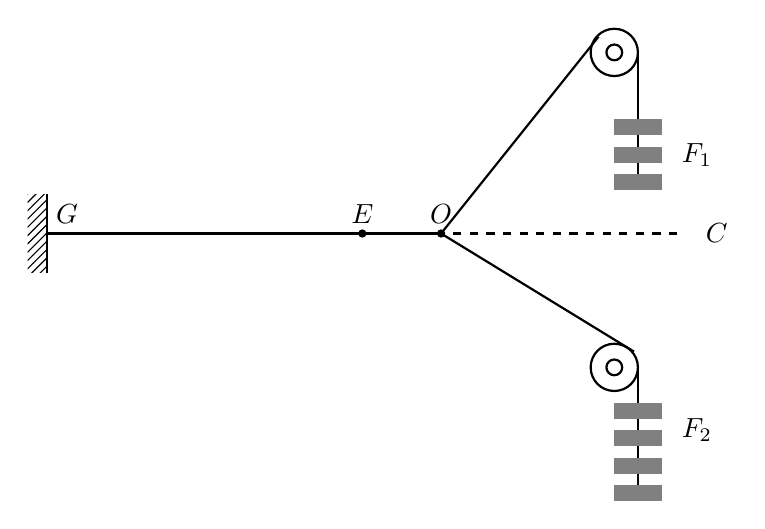
\begin{tikzpicture}[>=stealth, thick,scale=1]
  % \useasboundingbox(-1,-0.75)rectangle(3.7,1.4);
  \fill [pattern = north east lines] (0.75+1,0) rectangle (1+1,1);
  \draw (1+1,1)--(1+1,0);
  \draw (2,0.5)--(7,0.5);
  \node at (1.25+1, 0.75){$G$};
  \draw [dashed](10,0.5)--(7,0.5);
  \fill (6, .5) circle[radius=1.5pt];
  \fill (7, .5) circle[radius=1.5pt];
  \node at (6, 0.75){$E$};
  \node at (7, 0.75){$O$};
  \node at (10.5, 0.5){$C$};
  \draw (7, .5)--(9, 3); \draw (7, .5)--(9.45, -1);
  \draw (9.2, 2.8) circle [radius=0.3];
  \draw (9.2, -1.2) circle [radius=0.3];
  \draw (9.2, 2.8) circle [radius=.1];
  \draw (9.2, -1.2) circle [radius=.1];
  \draw(9.2+.3,2.8)--(9.2+.3,2.8-1.7);
  \draw(9.2+.3,-1.2)--(9.2+.3,-1.2-1.5);
  \foreach \x in {1,2,3}
  {
      \fill [black!50] (9.2,\x*.35+.7) rectangle (9.2+.6,\x*.35+0.2+.7);
  }
  \node at (10.25, 1.5){$F_1$};
  \foreach \x in {1,2,3,4}
  {
      \fill [black!50] (9.2,-\x*.35-1.5) rectangle (9.2+.6,-\x*.35+0.2-1.5);
  }
  \node at (10.25, -2){$F_2$};
\end{tikzpicture}
\end{document}